\documentclass{article}

\usepackage{url} 

\usepackage{pdfpages}
\usepackage{lastpage}
\usepackage{fancyhdr}
\usepackage{ngerman}


\usepackage{floatrow}
\usepackage[tableposition=top]{caption}
\floatsetup[table]{capposition=top}

\usepackage{amsmath, amssymb}

\usepackage[utf8]{inputenc}


\usepackage[numbib]{tocbibind}


\title{Oberflächenspannung}
\author{Johannes Winkler}
\date{}


\newcommand\twodigits[1]{%
   \ifnum#1<10 0#1\else #1\fi
}



\lhead{Oberflächenspannung}
\rhead{\today\\Johannes Winkler}
\cfoot{\twodigits{\thepage}~/ \pageref{LastPage}}

\begin{document}

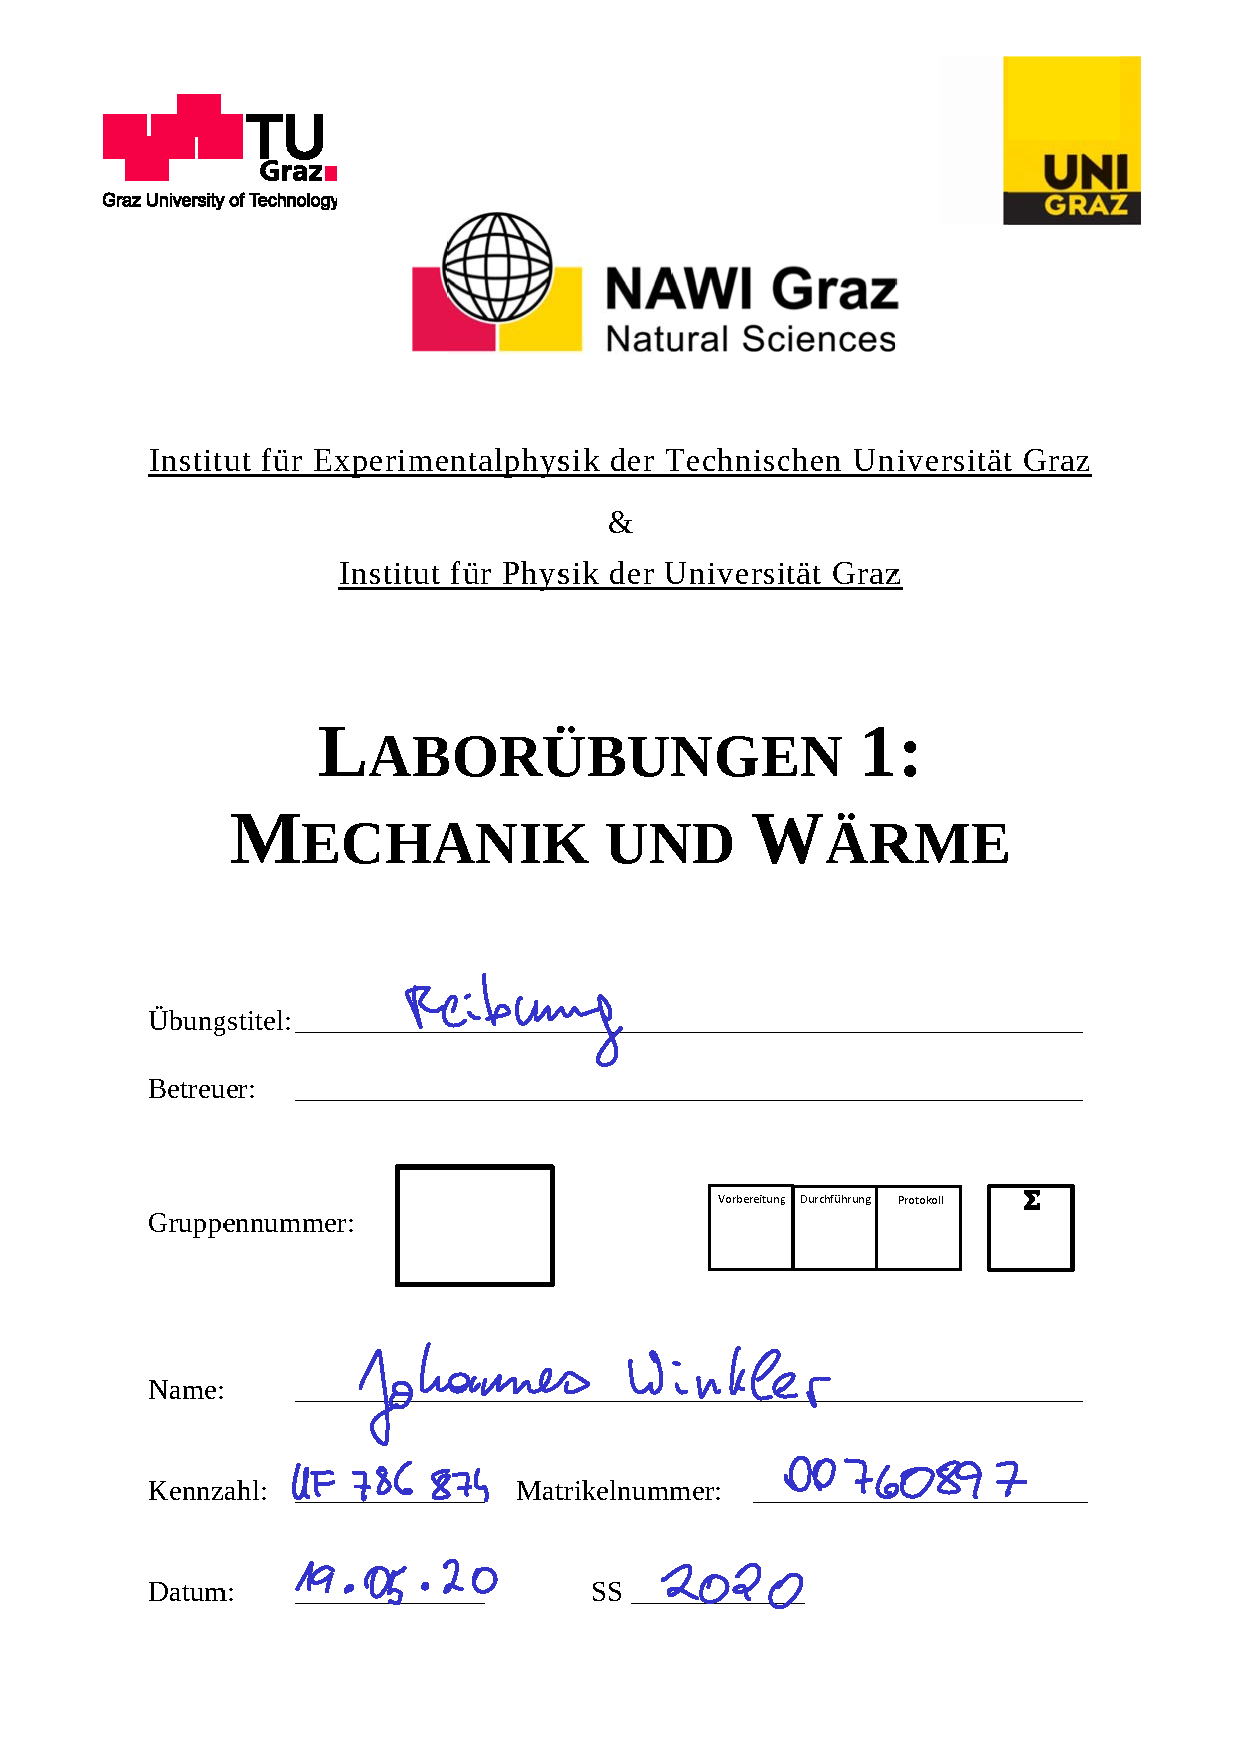
\includepdf[page=-]{deckblatt.pdf} 
 
 
\pagestyle{fancy}


\tableofcontents

\newpage


\setcounter{section}{-1}

\section{Experimentiervorschlag}


Ich möchte im Rahmen dieses Versuches die Koeffizienten der Haft-, Gleit- und Rollreibung verschiedener Gegenstände auf einer Oberfläche testen. 

Als schräge Unterlage würde ich eine bei IKEA gekaufte Laptop-Unterlage aus Plastik verwenden. 

\begin{figure}[H]
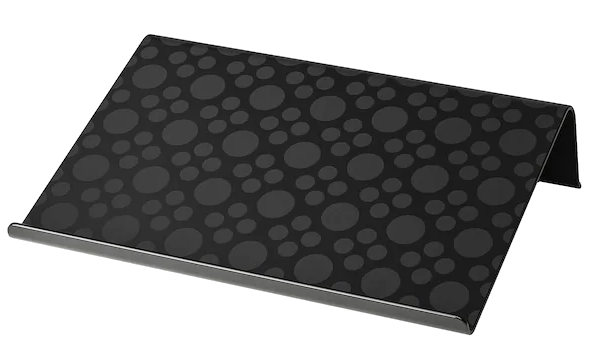
\includegraphics[height=5cm]{unterlage.png}
\caption{IKEA Laptop Unterlage}
\end{figure}

\begin{figure}[H]
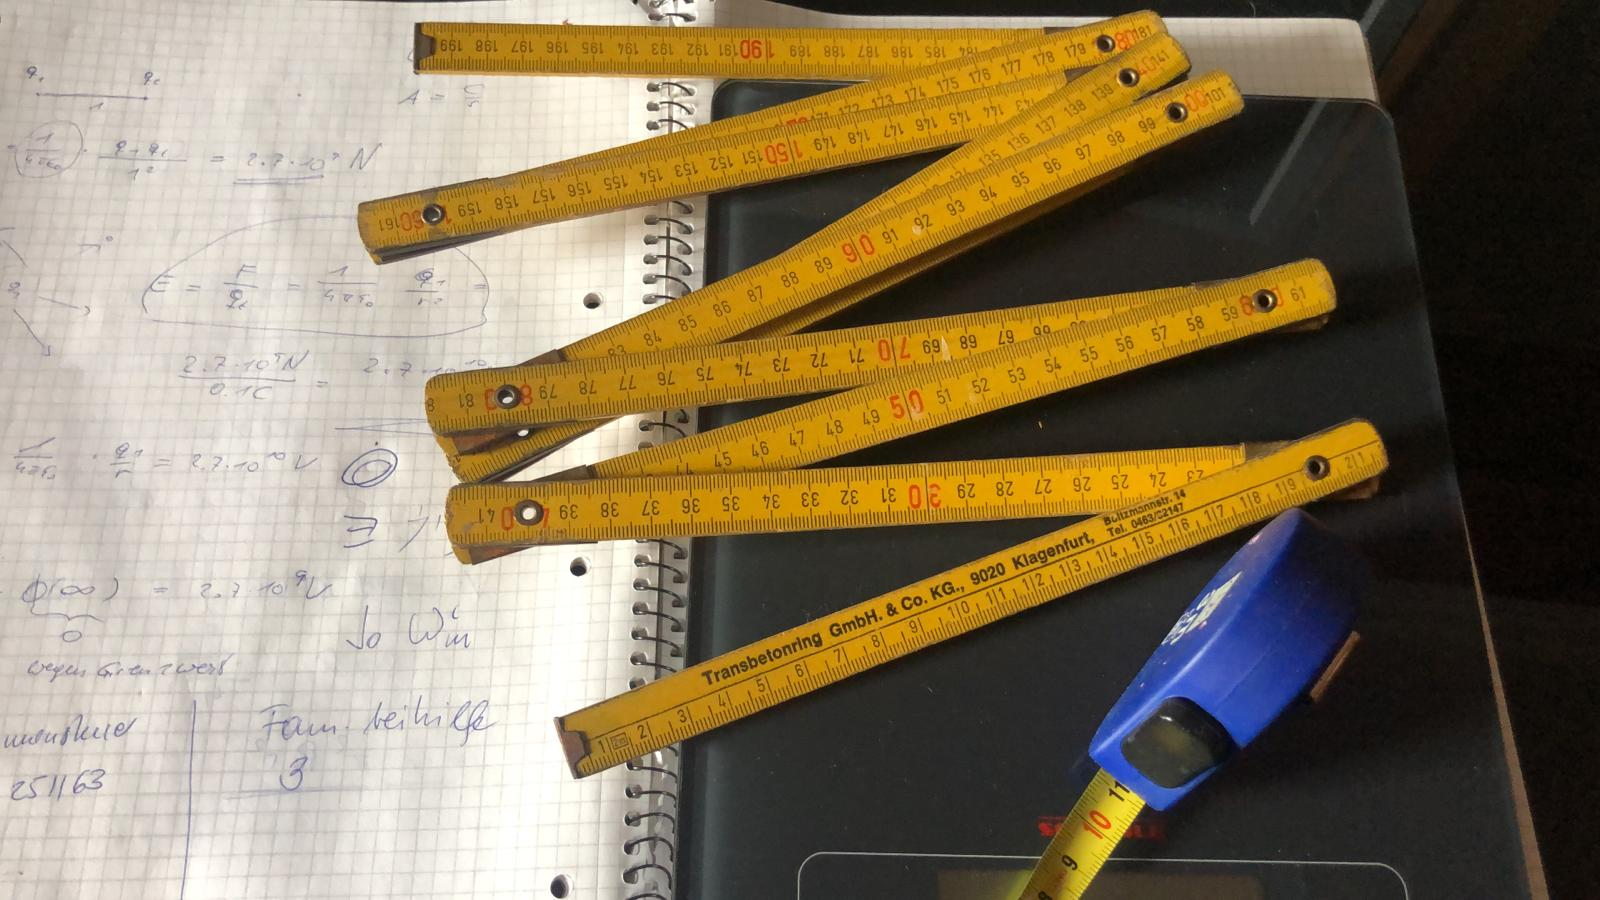
\includegraphics[height=5cm]{zeux.jpg}
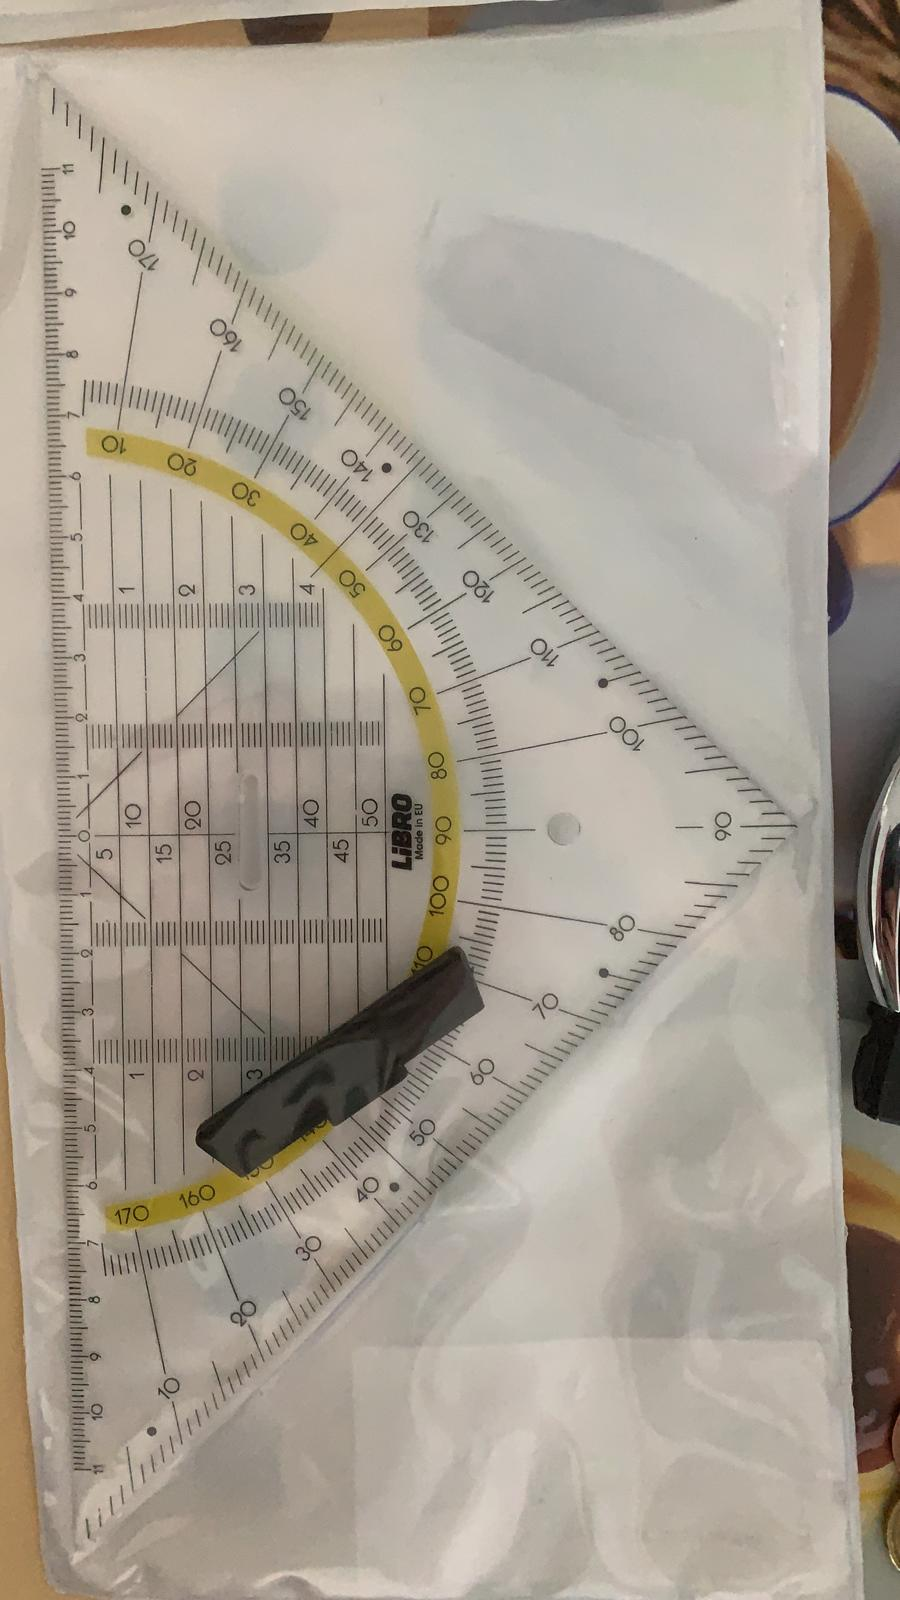
\includegraphics[height=5cm]{lineal.jpg}
\caption{Messinstrumente}
\end{figure}

Als Gegenstände möchte ich Münzen anhnad ihres Materials vergleichen. Also insbesondere ob es einen messbaren Unterschied zwischen Gold- und Kupfermünzen gibt.

Für die Rollreibung nehme ich Konservendosen für Lebensmitteln. Hier ist es insbesondere interessant, wie ich die Inhaltsmenge experimentell auf die Eigenschaften bei der Rollreibung auswirkt. 


\begin{figure}[H]
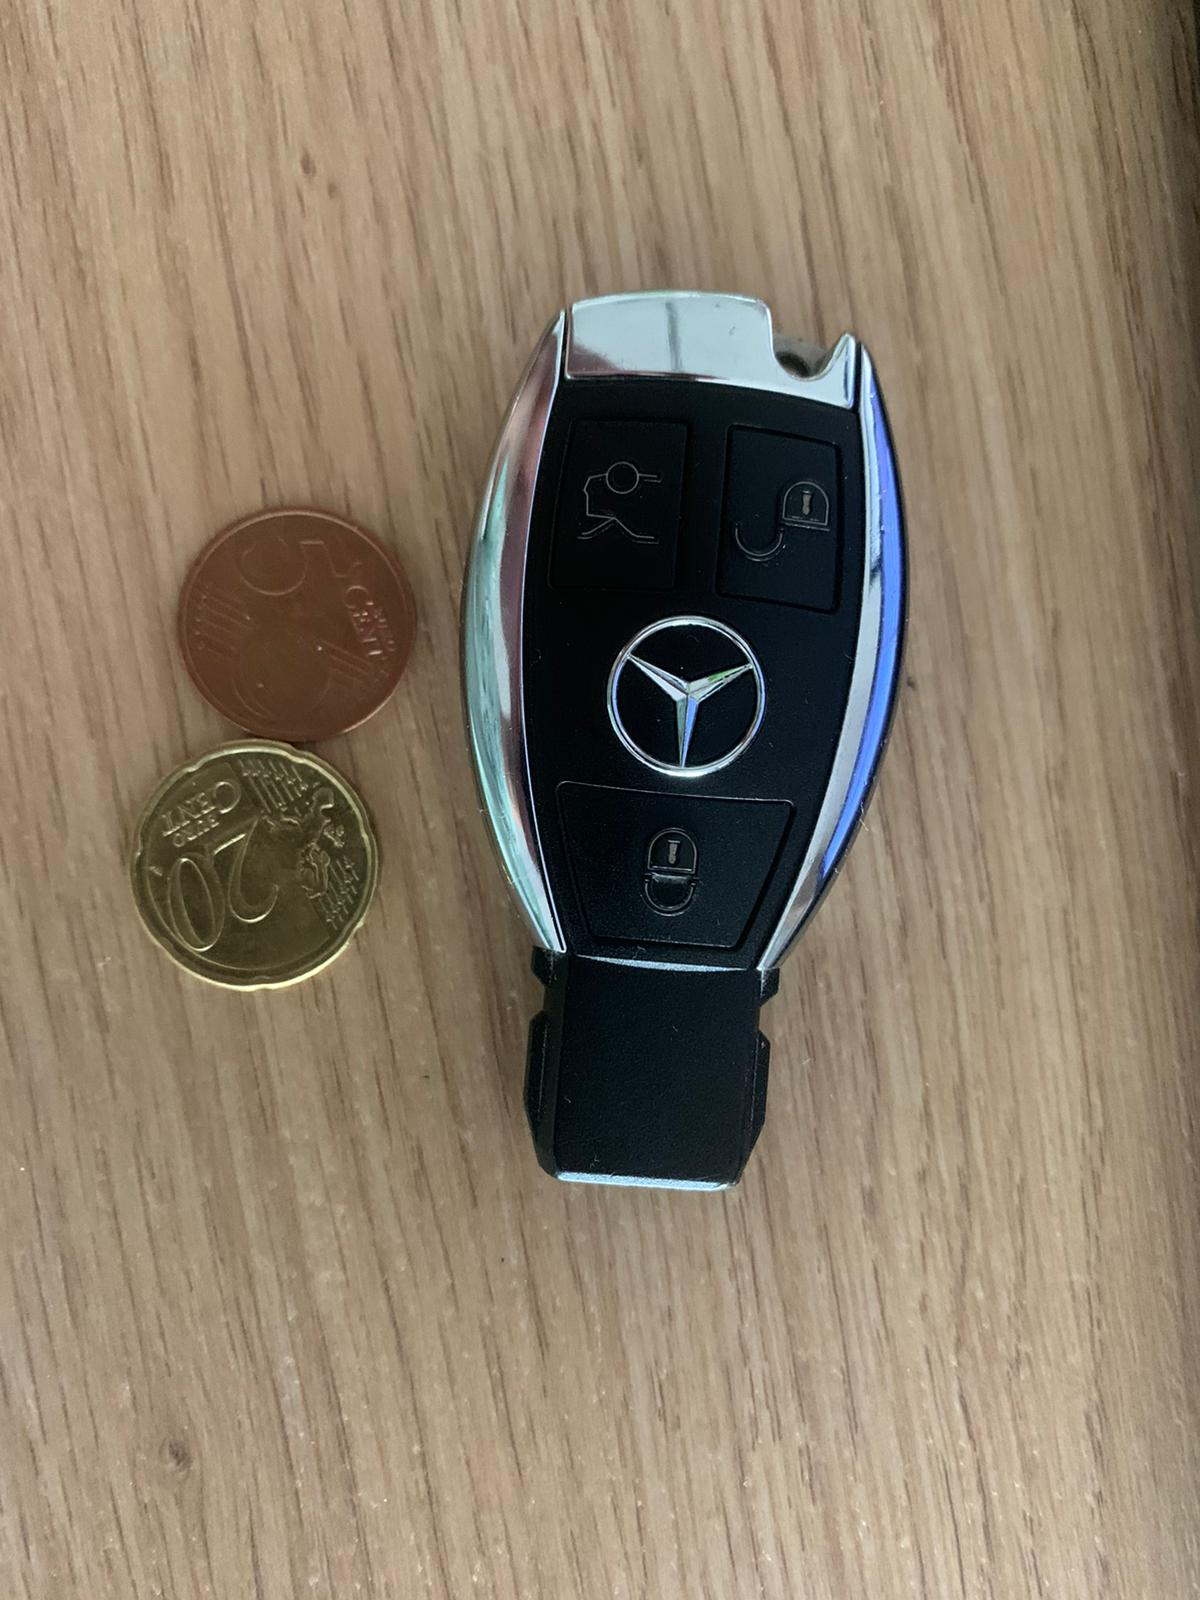
\includegraphics[height=5cm]{schlussel_muenzen.jpg}
\caption{Münzen und Autoschlüssel}
\end{figure}

\begin{figure}[H]
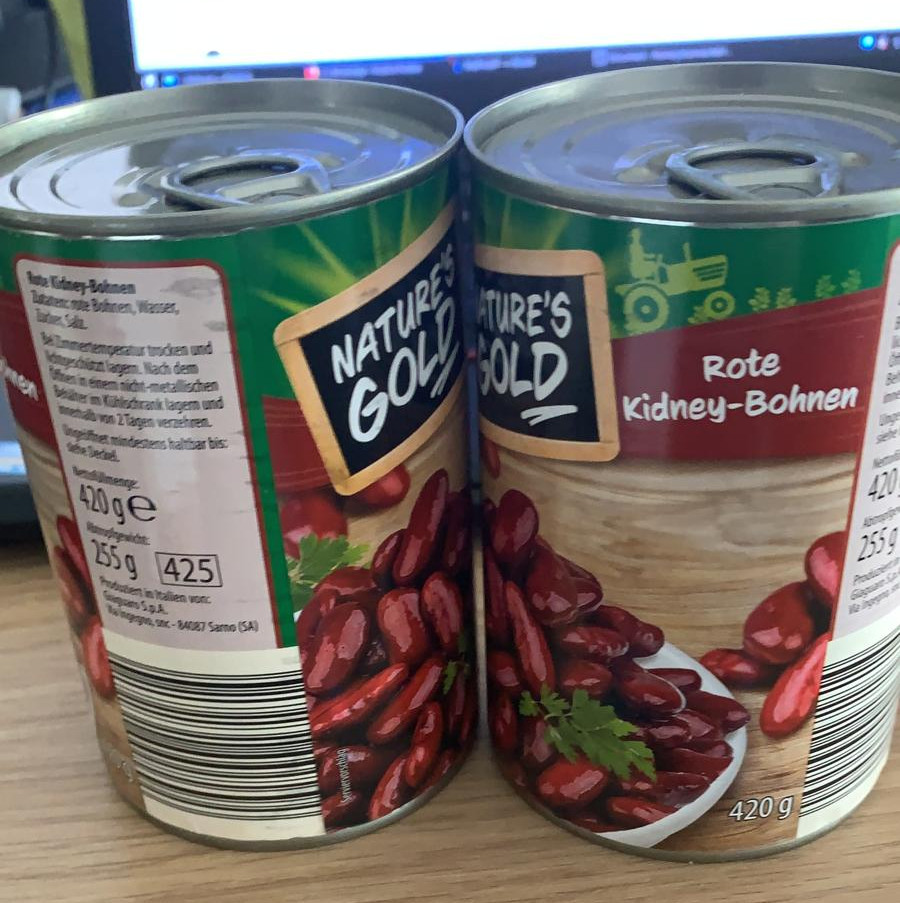
\includegraphics[height=5cm]{futter.jpg}
\caption{Dosen für die Messung von Rollreibung}

\end{figure}


Für das Experiment mit der Viskosität habe ich die Gegenstände am Zweitwohnsitz. Also Glaskugeln und (ungebrauchtes Motoröl). Könnte die Fotos dafür nachliefern. Bzw ich würde das Motoröl kaufen, wenn der Versuch genehmigt ist (40 Euro pro Packung).

\subsection{Kontrollfragen}
\begin{itemize}
\item Wie erfolgt die idealisierte Bewegung ohne Reibung?


Für die idealisierte Reibung setzt man 
\begin{align*}
\mu_R = \mu_G = \mu_H = 0
\end{align*}
Dadurch sind alle Reibungskräfte auf null.

\item Welche Reibung ist geschwindigkeitsunabhängig?

Haft-, Gleit- und Rollreibung sind unabhängig von der Geschwindigkeit weil diese nicht in der Formel vorkommt. 

\item Welche Reibung ist abhängig von der Geschwindigkeit?

Die Stokes-Reibung enthält die Geschwindigkeit in der Formel.


\item Wodurch entsteht Reibung?

mikroskopische Unenbenheiten auf den Oberflächen von Körpern

\item Was ist der Unterschied zwischen Haft- und Gleit-Reibung?

Haftreibung ist jene Kraft, die einen Körper auf einer schiefen Ebene im Stillstand hält.

\item Warum ist Gleitreibung meist kleiner als die Haftreibung?

Bei Stillstand sind die mikroskopischen Unebenheiten in den Ebenen \textit{verzahnt}. Diese zu lösen benötigt mehr Kraft.

\item Warum driften Ralley-Fahrer durch die Kurven und nicht Formel 1 Piloten?

Formel 1 ist mathematisch durchoptimiert. Bei der Formel 1 sind Reifen mit besseren Werten im Einsatz, sodass Driften nicht nötig ist (kostet Energie und Zeit). Dafür funktionieren Ralley Autos im Gelände, wo das F1 Auto nicht mehr lauffähig ist. Ist quasi eine Frage der Anwendung.

\item Was ist die Einheit der Viskosität?

\begin{align*}
\frac{\text{N}\cdot \text{s}}{\text{m}}
\end{align*}

\item Wie funktioniert ein Rotationsviskosimeter?

Ein technisches Gerät, dass durch Rotation eines mit Fluid gefüllten Zylinders die Viskosität des Fluids feststellen kann.


\item Was ist das Besondere der laminaren Strömung?

Es handelt sich um eine Strömung, in der keine Turbulenzen vorkommen. Man kann die Strömung in sich nicht vermischende Schichten einteilen.

\item Was ist die Reynolds Zahl und was bedeutet sie?

Verhältnis der kinitischen Energie eines infinitesimalen Volumens zur Reibungsenergie der Verschiebung. Diese Zahl kann genutzt werden um auf die Turbulenz einer Strömung zu schließen (Achtung: gibt auch andere Abhängigkeiten, zB Anfangsbedingungen, Beschaffenheit der Umbgebung et)

\end{itemize}

\newpage

\section{Aufgabenstellung}

Es soll der Haft-, Gleit- und Rollreibungskoeffizient bestimmt werden. Zusätzlich kann die Reibung in einer Flüssigkeit nach dem Stokes-Gesetz bestimmt werden.

\section{Grundlagen}

Bei der Haftreibung gilt, dass diese einen Körper auf einer schiefen Ebene in der momentanen Position hält. Man hat also eine Gegenkraft zum anteiligen Kraftvektor in Richtung der schiefen Ebene. Daher gilt laut Grafik \ref{fig:haftgleitreibung}
\begin{align}
\mu_H\cdot F_N &= m\cdot g \sin(\alpha) \\
\mu_H \cdot m\cdot g\cdot\cos(\alpha) &= m\cdot g \cdot \sin(\alpha) \\
\mu_h &= \tan(\alpha)
\end{align}
Um den maximalen Wert für $\mu_H$ zu erfahren, müssen wir jenen Wert $\alpha$ suchen, sodass sich der Körper zu bewegen beginnt. Daraus lässt sich der Haftreibungskoeffizient bestimmen.

Den Gleitreibungskoeffizienten findet man durch die Differenz von der parallelen Komponente der Gewichtskraft und der Reibungskraft
\begin{align}
m\cdot a &= F_g\cdot \sin(\alpha) - \mu_G \cdot F_N \\
m\cdot a &= m\cdot g\cdot \sin(\alpha) - \mu_G \cdot m\cdot g\cdot \cos(\alpha)\\
 a &= g\cdot \sin(\alpha) - \mu_G \cdot g\cdot \cos(\alpha) \\
  \mu_G &= \frac{\sin(\alpha) - \frac{a}{g}}{\cos(\alpha)}
\end{align}
Mit $s = \frac{a\cdot t^2}{ 2}$ ergibt sich
\begin{align}
\mu_G = \frac{\sin(\alpha) - \frac{2\cdot s}{g\cdot t^2}}{\cos(\alpha)}
\label{eq:gleitreibung}
\end{align}
Theoretisch lässt sich der Haftreibungskoeffizient aus $\mu_G$ bestimmen, wenn man diesen für $s\to 0$ und $t\to\infty$ setzt.

\begin{figure}[H]
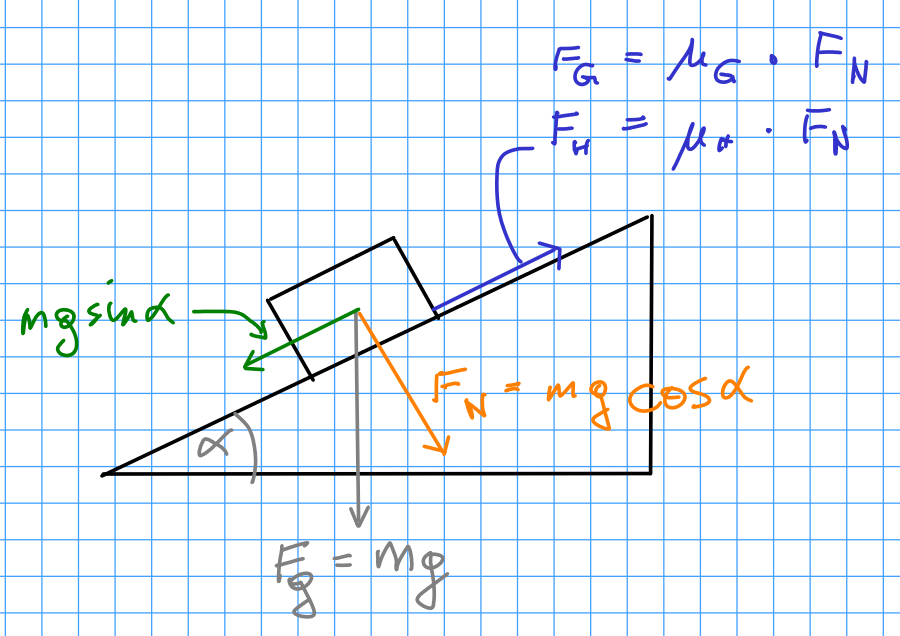
\includegraphics[height=6cm]{reibung1.png}
\caption{Haft- und Gleitreiung}
\label{fig:haftgleitreibung}
\end{figure}



Für die Rollreibung gilt
\begin{align}
\mu_R = \frac{F_R}{F_N}\cdot r
\end{align}
\begin{figure}[H]
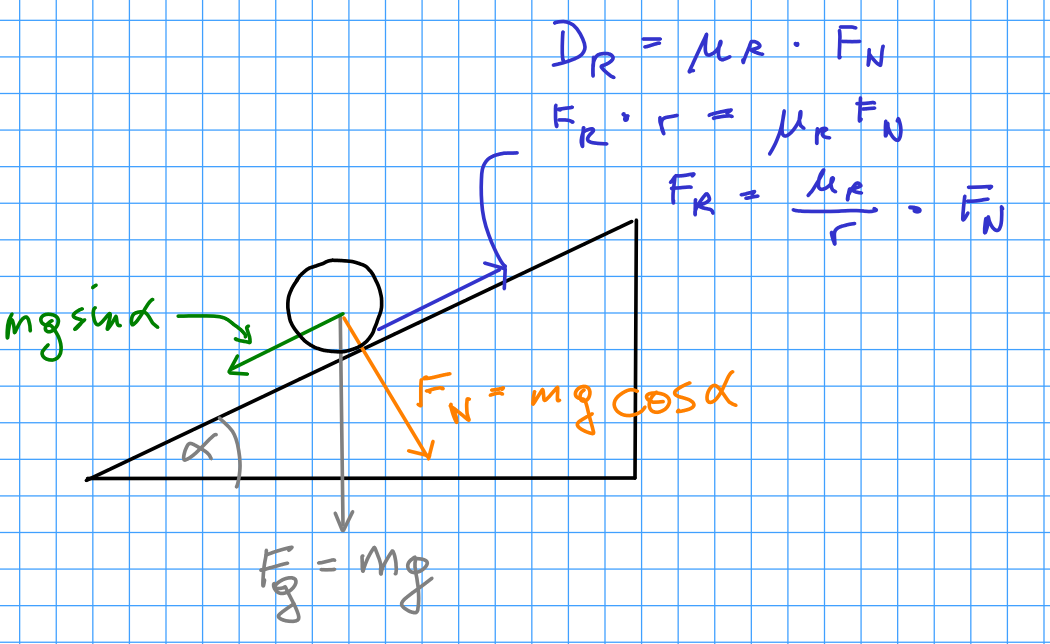
\includegraphics[height=5cm]{reibung2.png}
\caption{Rollreiung}
\label{fig:rollreibung}
\end{figure}


Für die Viskosität wird das Stokes'sche Gesetz benötigt. (vgl. \cite{demtr1})
\begin{align}
F_{\text{Stokes}} = -6\cdot \pi \cdot \eta \cdot r \cdot v
\end{align}

Gemäß Grafik \ref{fig:stokes} muss man die Kräfte folgend addieren
\begin{align*}
F_{\text{Schwerkraft}} - F_{\text{Auftrieb}} - F_{\text{Stokes}} &= 0 \\
(\rho_K - \rho_{\text{Fluid}})\cdot \frac{4\cdot \pi}{3} \cdot r^3 \cdot g &= 6\cdot \pi \cdot \eta \cdot r\cdot v \\
(\rho_K - \rho_{\text{Fluid}})\cdot \frac{2\cdot r^2 }{9 \cdot v} \cdot g &= \eta 
\end{align*}



\begin{figure}[H]
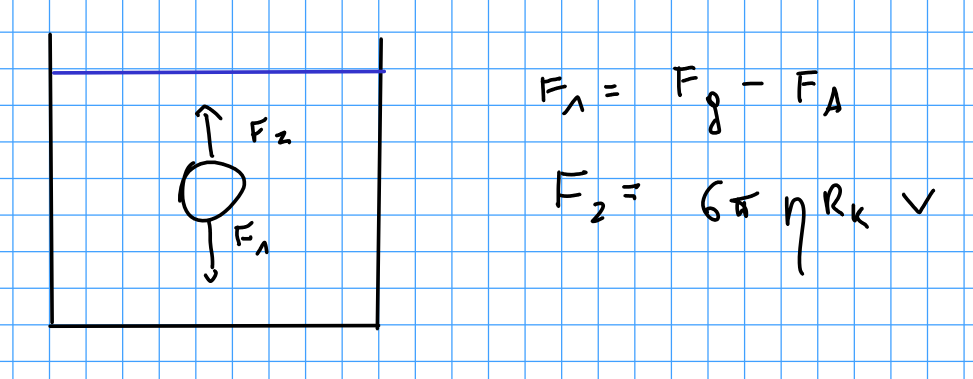
\includegraphics[height=4cm]{stokes.png}
\caption{Stokes'sche Reibung}
\label{fig:stokes}
\end{figure}


\newpage

\section{Beschreibung der Versuchsanordnung}

Im wesentlichen ist der Versuch in den Abbildungen \ref{fig:haftgleitreibung}, \ref{fig:rollreibung} und \ref{fig:stokes} gezeigt. 





\section{Geräteliste}



\begin{table}[H]
\caption{Geräteliste}



\begin{tabular}{lll}
Gerät  & Beschreibung \\
\hline
Münzen  & übliche Euromünzen (Herkunftsland separat angegeben) \\
Autoschlüssel & Marke: Mercedes-Benz \\
Laptop Unterlage BRÄDA & gekauft bei IKEA, interne IKEA-Artikelnummer:  601.501.76 \\
Geodreieck & Länge 25 cm, von der Libro Eigenmarke \\
Küchenwaage & von Firma Soehnle, digitales Display, Maximalgewicht 5~kg \\
Stoppuhr / Kamera & iPhone XS Max \\
2 Dosen rote Kidney Bohnen & voll und leer 
\end{tabular}
\end{table}

\newpage
\section{Versuchsdurchführung und Messergebnisse}

Für Haft- und Gleitreibung wird jeweils eine 20 Cent und eine 5 Cent Münze verwendet. 


\subsection{Haftreibung}



\begin{table}[H]
\caption{Messwerte für Haftreibung}
\begin{tabular}{l|rr}
Nr. & \shortstack[l]{Winkel bei\\20 Cent Münze / ${}^\circ$} & \shortstack[l]{Winkel bei\\5 Cent Münze / ${}^\circ$} \\
\hline
1 & 24 & 25 \\
2 & 19 & 26 \\
3 & 19 & 26 \\
4 & 23 & 22 \\
5 & 20 & 21 \\
6 & 23 & 24 \\
7 & 19 & 22 \\
8 & 26 & 21 \\
9 & 23 & 18 \\
10 & 19 & 23 \\
11 & 19 & 18 \\
12 & 18 & 23 \\
13 & 24 & 23 \\
14 & 24 & 25 \\
15 & 19 & 25 \\
16 & 22 & 19 \\
17 & 26 & 21 \\
18 & 21 & 19 \\
19 & 19 & 26 \\
20 & 21 & 18 \\
\hline
$\overline{X}$ & 21.4 & 22.25

\end{tabular}
\end{table}

\newpage

\subsection{Gleitreibung}

Für die Gleitreibung wird Zeit, Strecke und Winkel benötigt. Die zurückgelegte Strecke ist in allen Fällen gleich, nämlich $s=42~$cm. Wir setzen den Winkel $\alpha=30^\circ$, sodass wir aufgrund der Zeitmessung den Gleitreibungskoeffizienten bestimmen können. Wichtig ist, dass der Winkel größer als jener bei der Haftreibung ist, da ansonsten die Münzen nicht zu rutschen beginnen. Der Gleitreibungskoeffizient berechnet sich nach Formel \eqref{eq:gleitreibung}. 


\begin{table}[H]
\caption{Messwerte für Gleitreibung}
\begin{tabular}{l|rr}
Nr. & \shortstack[l]{Zeit bei\\ 20 Cent Münze / s} & \shortstack[l]{Zeit bei \\ 5 Cent Münze/ s} \\
\hline
1 & 0.29 & 0.83 \\
2 & 0.53 & 0.53 \\
3 & 0.92 & 0.43 \\
4 & 0.67 & 0.64 \\
5 & 0.64 & 0.63 \\
6 & 0.49 & 0.54\\
7 & 0.51 & 0.62\\
8 & 0.55 & 0.66\\
9 & 0.60 & 0.68\\
10 & 0.68 & 0.51\\
11 & 0.73 & 0.62\\
12 & 0.64 & 0.58\\
13 & 0.64 & 0.66\\
14 & 0.76 & 0.82\\
15 & 0.64 & 0.55\\
16 & 0.49 & 0.53\\
17 & 0.37 & 0.74\\
18 & 0.56 & 0.64\\
19 & 0.51 & 0.75\\
20 & 0.46 & 0.54\\
\hline 
$\overline{X}$ & 0.584 & 0.614
\end{tabular}
\end{table}







\subsection{Rollreibung}


\begin{table}[H]
\caption{Messwerte für Rollreibung}
\begin{tabular}{l|rr}
Nr. & \shortstack[l]{Winkel bei\\voller Dose Münze / ${}^\circ$} & \shortstack[l]{Winkel bei\\leerer Dose  / ${}^\circ$} \\
\hline
1 & 12 & 13 \\ 
2 & 11 & 16 \\ 
3 & 13 & 10 \\ 
4 & 8 & 10 \\ 
5 & 8 & 11 \\ 
6 & 13 & 10 \\ 
7 & 7 & 13 \\ 
8 & 14 & 12 \\ 
9 & 11 & 12 \\ 
10 & 13 & 13 \\ 
11 & 9 & 11 \\ 
12 & 12 & 11 \\ 
13 & 11 & 10 \\ 
14 & 13 & 8 \\ 
15 & 7 & 10 \\ 
16 & 7 & 9 \\ 
17 & 9 & 13 \\ 
18 & 14 & 16 \\ 
19 & 7 & 14 \\ 
20 & 14 & 13 \\
\hline
$\overline{X}$ & 10.65 & 11.75
\end{tabular}
\end{table}





\subsection{Viskosität}

Aus technischen Gründen (Motoröl wurde bereits ins Motorrad geschüttet), werde ich den gegebenen Datensatz auswerten. Es wird eine Stahlkugel ins Speiseöl getaucht, sodass diese mit konstanter Geschwindigkeit einsinkt. Der Durchmesser der Kugel ist $d = 1.05$ mm. Es wird die benötigte Zeit für die Fallhöhe $h=500$ mm gemessen. Für die Dichte von Stahl und Speiseöl beziehen wir aus der Literatur die Werte $\rho_{\text{Stahl}} = 7850$ kg m${}^{-3}$ und  $\rho_{\text{Öl}} = 920$ kg m${}^{-3}$.

\begin{table}[H]
\caption{Messwerte für Viskosität}
\begin{tabular}{lrr}
Nr. & \shortstack[l]{Zeit / s} & Viskosität / mPa s\\
\hline
1 & 10.70 & 89.1091 \\
2 & 10.72 & 89.2757\\
3 & 10.67 & 88.8593\\
4 & 10.90 & 90.7747\\
5 & 10.84 & 90.2750 \\
\hline
$\overline{X}$ & 10.766 & 89.6588
\end{tabular}
\end{table}




\newpage
\section{Auswertung}

\subsection{Plots}


\begin{figure}[H]
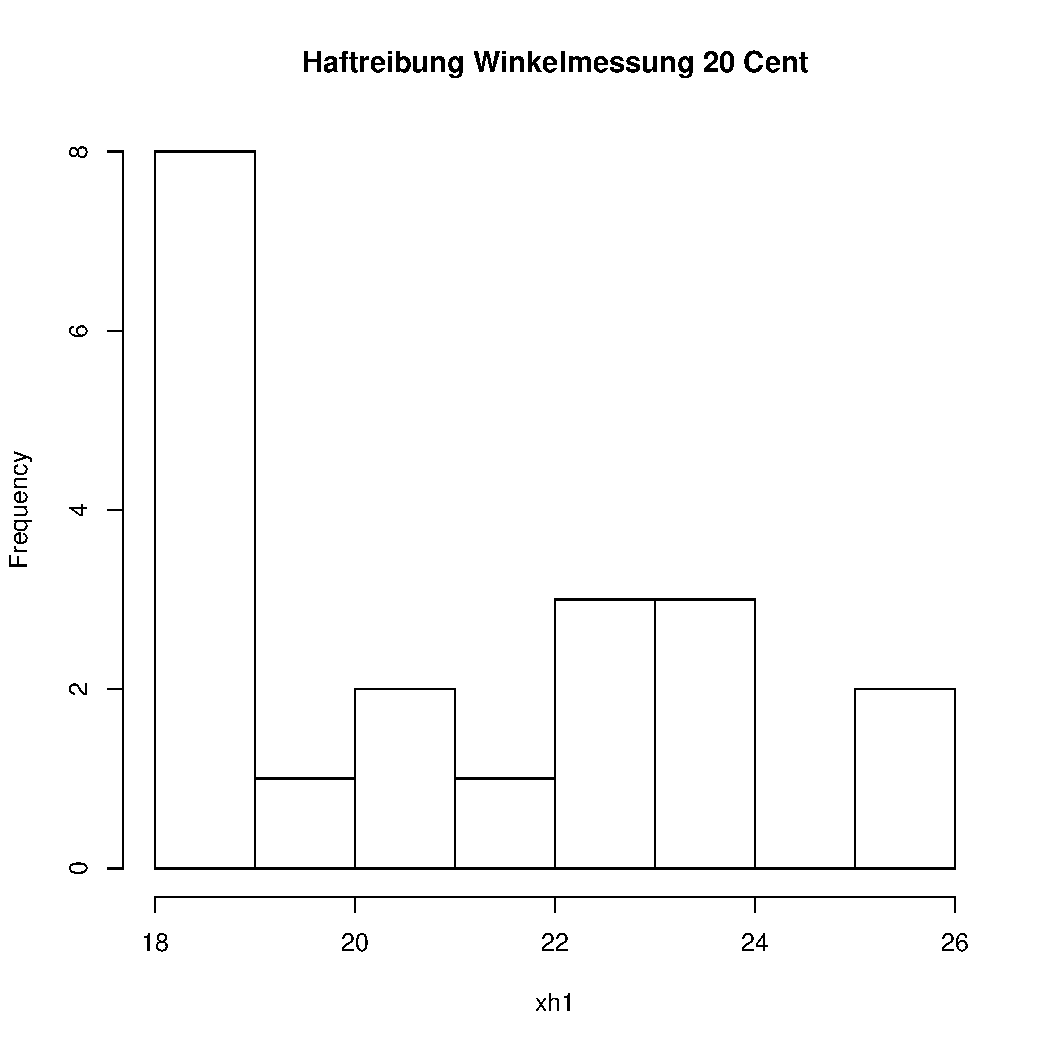
\includegraphics[width=.45\textwidth]{Haft_20_cent.pdf}
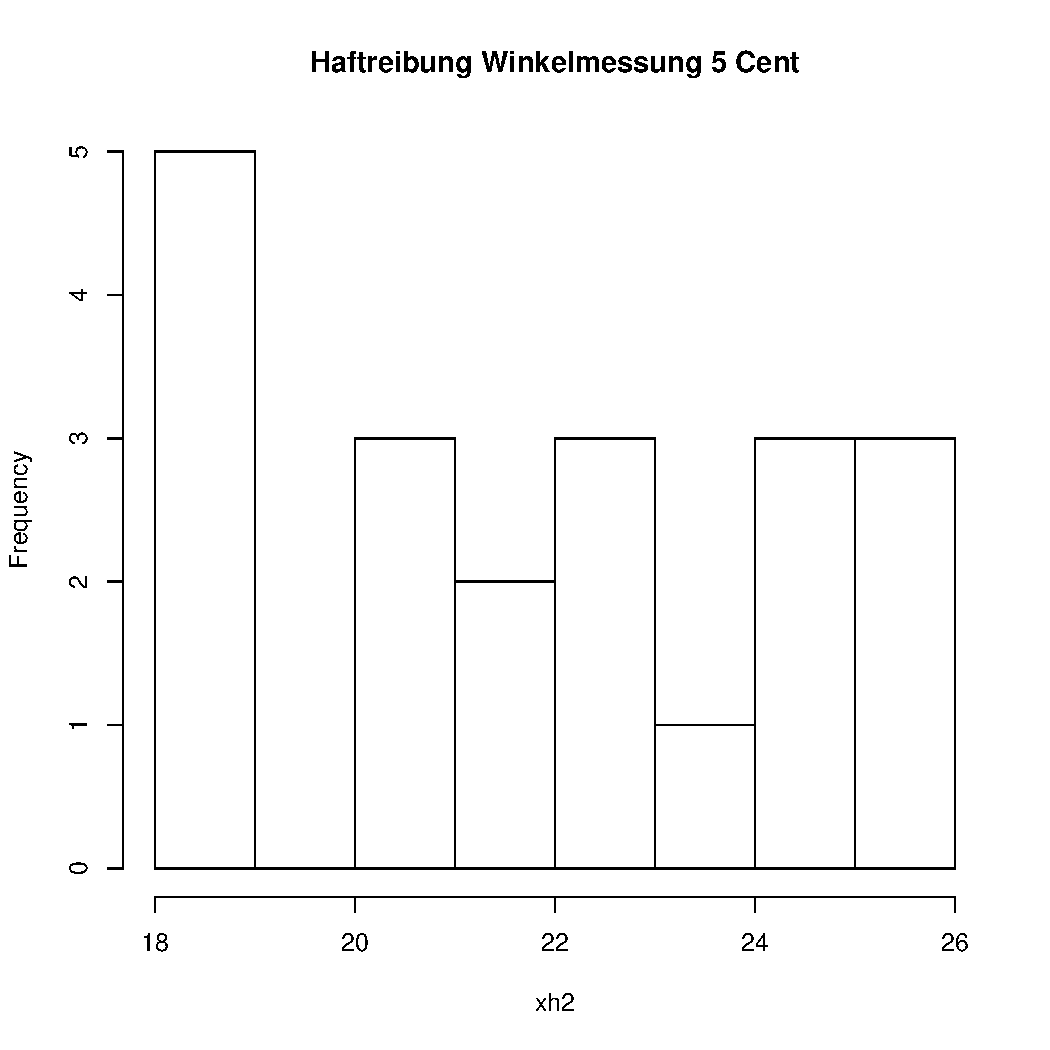
\includegraphics[width=.45\textwidth]{Haft_5_cent.pdf}

\caption{Histogramm für gemessenen Winkel bei Haftreibung in Grad.}
\end{figure}



\begin{figure}[H]
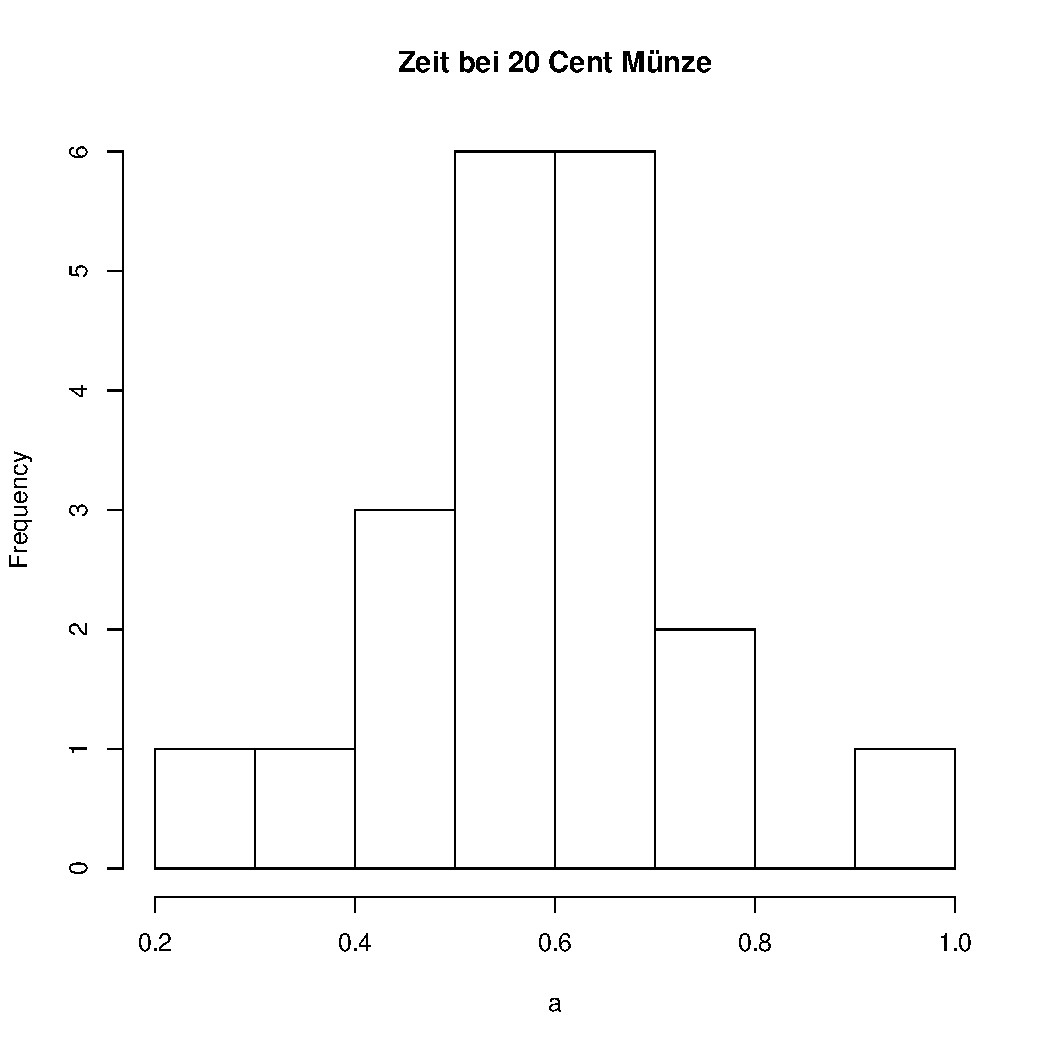
\includegraphics[width=.45\textwidth]{Gleitreibung_20_cent.pdf}
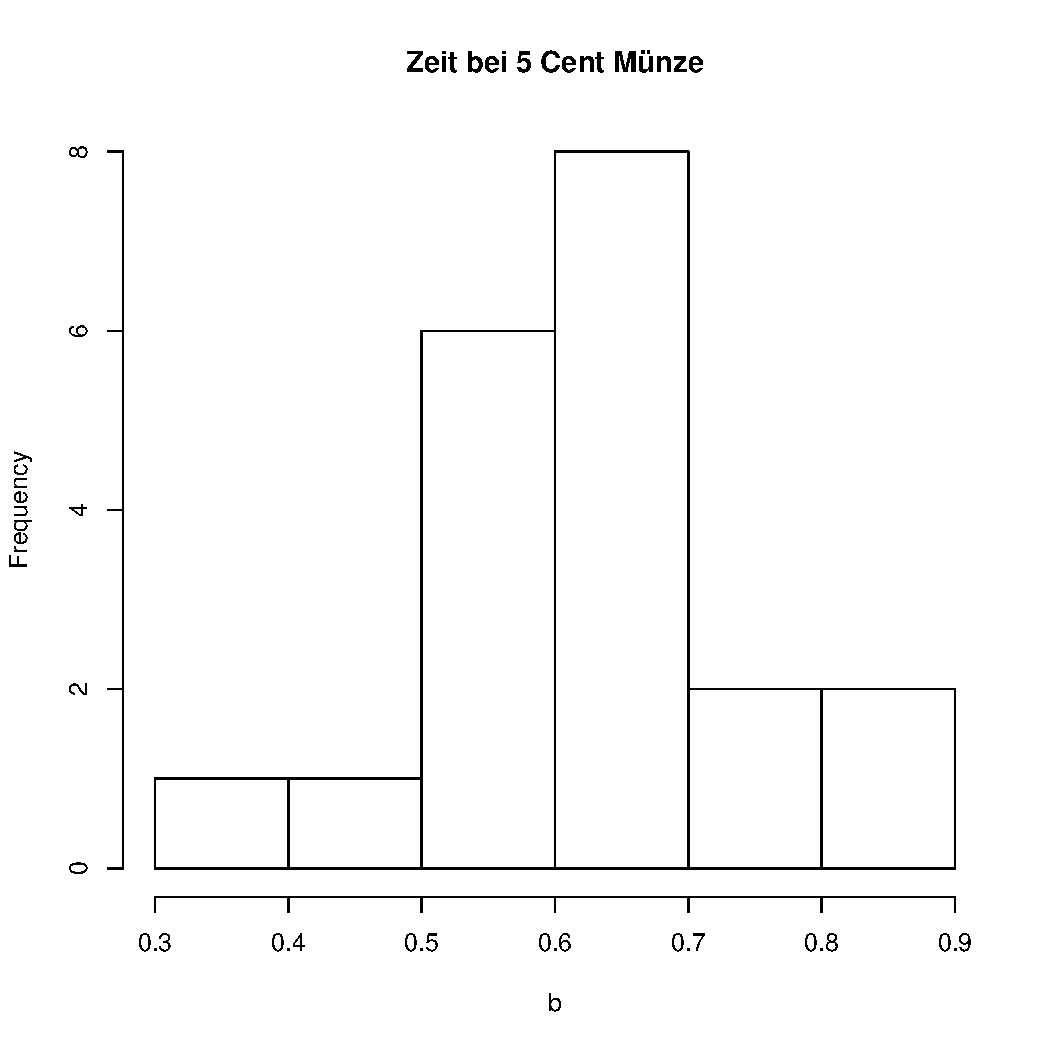
\includegraphics[width=.45\textwidth]{Gleitreibung_5_cent.pdf}

\caption{Histogramm für Zeiten bei Gleitreibung in Sekunden.}
\end{figure}


\begin{figure}[H]
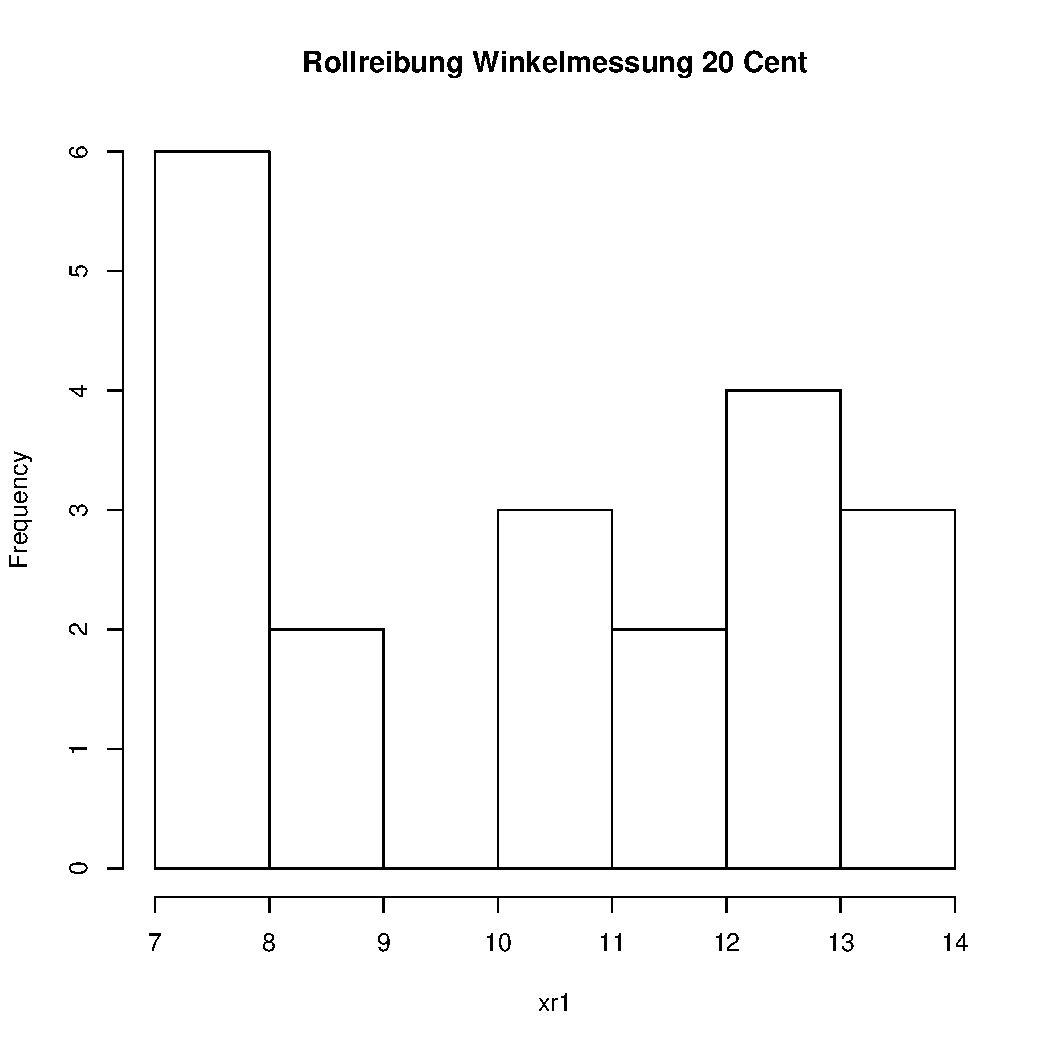
\includegraphics[width=.45\textwidth]{Roll_20_cent.pdf}
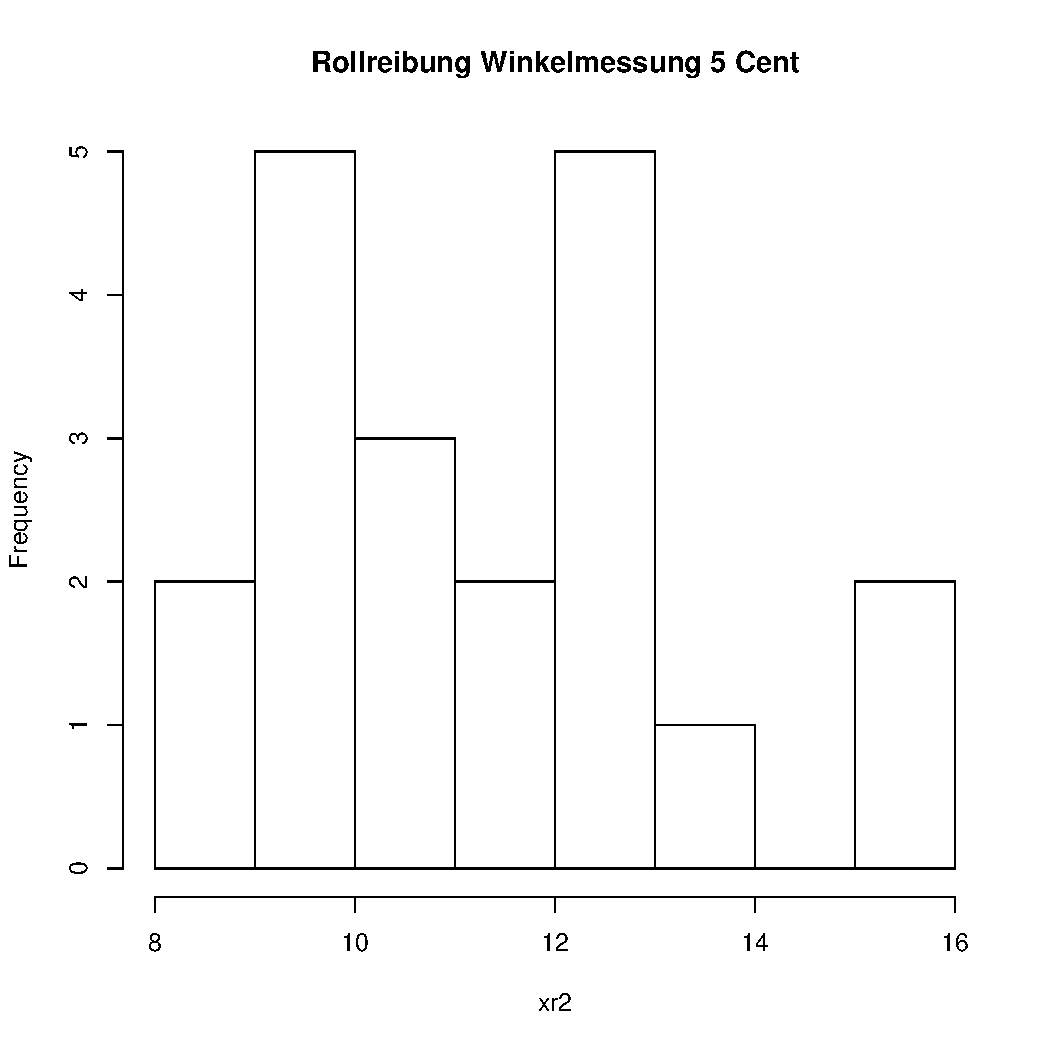
\includegraphics[width=.45\textwidth]{Roll_5_cent.pdf}

\caption{Histogramm für gemessenen Winkel bei Rollreibung in Grad.}
\end{figure}


\subsection{Größtunsicherheitsmethode}

Der Haftreibungskoeffizient ist nur vom Winkel $\alpha$ abhängig. Es gilt
\begin{align}
\mu_H = \tan(\alpha)
\end{align}
wobei $\alpha$ jener Winkel ist, sodass sich das Objekt zu bewegen beginnt. Für die Abmessung mit dem Geodreieck nehme ich einen Messfehler von $\Delta\alpha = 2^\circ$ an wobei das Bogenmaß angegeben werden muss, also $\Delta\alpha = \frac{\pi}{90}$.
Es gilt für die Gesamtunsicherheit
\begin{align}
\Delta\mu_H &= \left|\frac{\partial \mu_H}{\partial \alpha}\right| \cdot \Delta \alpha = \frac{\Delta\alpha}{\cos^2(\alpha) } = \frac{\pi}{90\cdot \cos^2(\alpha)}
\end{align}


Für den Gleitreibungskoeffizienten gilt
\begin{align}
\mu_G = \frac{\sin(\alpha) - \frac{2\cdot s}{g\cdot t^2}}{\cos(\alpha)}
\end{align}
Dessen Unsicherheit ist 
\begin{align}
&\Delta\mu_G = \left|\frac{\partial \mu_G}{\partial \alpha}\right| \cdot \Delta\alpha + \left|\frac{\partial\mu_G}{\partial s}\right| \cdot \Delta s + \left|\frac{\partial\mu_G}{\partial t}\right| \cdot \Delta t \\
&= \left| \frac{1 - \frac{2\cdot s}{g\cdot t^2} \cdot \sin(\alpha)}{\cos^2(\alpha)}\right|\cdot \Delta\alpha + \left| \frac{2}{g\cdot t^2\cdot \cos(\alpha)} \right| \cdot \Delta s + \left| \frac{4\cdot s}{g\cdot t^3\cdot \cos(\alpha)} \right| \cdot \Delta t
\end{align}



Numerisch ergibt sich für die Unsicherheit der Gleitreibung 
\begin{align}
\Delta\mu_{G} &= \left| \frac{1 - \frac{0.42}{9.81\cdot t^2} }{0.75}\right|\cdot \frac{\pi}{90} + \left| \frac{0.235413}{t^2} \right| \cdot \Delta s + \left| \frac{0.197747}{t^3} \right| \cdot \Delta t
\end{align}
wobei hierfür $\alpha=30^\circ$, $\Delta \alpha = \pi/90$ gegeben sind. Die Messfehler für Zeit und Länge nehmen wir als $\Delta s = 0.001$~m und $\Delta t = 0.1$~s an. Insgesamt ergeben die Unsicherheiten 
\begin{align}
\Delta\mu_{G,\text{20 Cent}} &= 0.1407 \\
\Delta\mu_{G,\text{5 Cent}} &= 0.1273 
\end{align}
Der mittlere Gleitreibungskoeffizient wäre nach \eqref{eq:gleitreibung}.
\begin{align}
\mu_{G,\text{20 Cent}} &= \frac{\sin\left(30^\circ\right) - \frac{2\cdot 0.42}{9.81\cdot 0.584^2}}{\cos\left(30^\circ\right)} = 0.2874 \\
\mu_{G,\text{5 Cent}} &= \frac{\sin\left(30^\circ\right) - \frac{2\cdot 0.42}{9.81\cdot 0.614^2}}{\cos\left(30^\circ\right)} = 0.3151
\end{align}

Für die Rollreibung ergibt sich analog zur Haftreibung
\begin{align}
\Delta\mu_R &= \left|\frac{\partial \mu_R}{\partial \alpha}\right| \cdot \Delta \alpha = \frac{\Delta\alpha}{\cos^2(\alpha) } = \frac{\pi}{90\cdot \cos^2(\alpha)}
\end{align}
wobei $\alpha$ jener Winkel ist, wo das Objekt zu rollen beginnt.




Für die Unsicherheit der Viskosität gilt
\begin{align}
\eta = (\rho_K - \rho_{\text{Fluid}}) \cdot \frac{2\cdot g}{9 }\cdot \frac{r^2 \cdot t}{h}
\end{align}
Die Unsicherheit ergibt
\begin{align}
\Delta\eta &= \left|\frac{\partial\eta}{\partial r}\right|\cdot \Delta r + \left|\frac{\partial\eta}{\partial t}\right|\cdot \Delta t + \left|\frac{\partial\eta}{\partial h}\right|\cdot \Delta h \\
&= (\rho_K - \rho_{\text{Fluid}})\cdot \frac{2\cdot g}{9} \cdot \left(\frac{2\cdot r \cdot \Delta r\cdot t}{h} + \frac{r^2\cdot\Delta t}{h} + r^2\cdot t \cdot |\log(h)| \cdot \Delta h \right) \\
&= 15107.4 \cdot \left(2.2609\cdot 10^{-6}  + 5.5125\cdot 10^{-8} + 4.1137\cdot 10^{-9}  \right)~\frac{\text{kg}}{\text{m s} } \\
&\approx 0.03505~\frac{\text{kg}}{\text{m s} } 
\end{align}

\newpage
\section{Zusammenfassung und Diskussion}


Für die Haftreibung ergibt sich für die 20 Cent bzw. für die 5 Cent Münze folgenes
\begin{align}
\mu_{H,\text{20 Cent}} &= \left(\tan\left(21.4)^\circ\right) \pm \frac{\pi}{90\cdot \cos^2\left(21.4^\circ\right)} \right) =& (0.3919 \pm 0.0403) \\
\mu_{H,\text{5 Cent}} &= \left(\tan\left(22.25)^\circ\right) \pm \frac{\pi}{90\cdot \cos^2\left(22.25^\circ\right)} \right) =& (0.4091 \pm 0.0407) 
\end{align}

Gemäß des Versuchsausganges besitzt die 20 Cent Münze einen geringen Haftreibungskoeffizienten, wobei aufgrund der Unsicherheiten dieses Ergebnis nicht eindeutig verifziert werden kann. Hier bräuchte man genauere Messinstrumente.

Für die Gleitreibung ergeben sich das Messergebnis mit den Unsicherheiten
\begin{align}
\mu_{G,\text{20 Cent}} &= \left(0.2874 \pm 0.1407\right) \\
\mu_{G,\text{5 Cent}} &= \left(0.3151 \pm 0.1273\right)
\end{align}
Die hohe Abweichung kommt durch die Zeitmessung zustande. Hier ist die Zeit als dritte Potenz im Nenner. Bei Messungen von unter einer Sekunde ergibt sich daher eine sehr große Ungenauigkeit.

Für die Rollreibung ergibt sich
\begin{align}
\mu_{R,\text{volle Dose}} &= \left(\tan\left(10.65^\circ\right) \pm \frac{\pi}{90\cdot \cos^2\left(10.65^\circ\right)} \right) =& \left(0.1880 \pm 0.0361\right) \\
\mu_{R,\text{leere Dose}} &= \left(\tan\left(11.75^\circ\right) \pm \frac{\pi}{90\cdot \cos^2\left(11.75^\circ\right)} \right) =& \left(0.2080 \pm 0.0365\right)
\end{align}
Hier besagt die Theorie laut \cite{demtr1} und \cite{giancoli}, dass der Rollreibungskoeffizient nicht von der Masse des Objektes abhängt. Experimentell zeigt sich, dass die volle Dose (also jene mit mehr Masse) geringfügig weniger Reibung besitzt. Allerdings liegt das im Rahmen der Unsicherheit und kann daher nicht mit hinreichender Genauigkeit bestimmt werden. 

Die Unsicherheit des Viskosität beträgt
\begin{align}
\eta = (89.6588 \pm 35.0507)~\frac{\text{g}}{\text{m s}}
\end{align}


Alles in allem bräuchte man bessere Hilfsmittel um genauer messen zu können. Insbesondere für die Gleitreibung wäre ein Versuchsaufbau mit einer Strecke von mehreren Metern sinnvoll. Dies ist in meiner Wohnung jedoch nicht möglich.


\begin{thebibliography}{9}
\bibitem{demtr1} W. Demtröder, \emph{Experimentalphysik 1: Mechanik und Wärme}, Springer-Spektrum, 8. Auflage, 2018.

\bibitem{giancoli} D. Giancoli, \emph{Physik}, Pearson, 4. Auflage, 2019.

\end{thebibliography}

\end{document}
